This chapter is devoted to an analysis of the functional and timing models in
SST when using the GPU component as a part of a generalized compute node. Since
GPUs in HPC function solely as co-processors, functionally executing GPU-enabled
binaries requires the CPU to initialize and launch kernels of work to the GPU.
Figure~\ref{fig:sst_volta} shows the general simulation model used for the evaluation.
The Command Link and Data Link serve as the transport mechanism for the CPU (host)
to launch and coordinate work with the GPU (device). The other components in each
model can be tailored to fit any host and device that one wishes to model.

   \begin{figure}[!htb]
      \centering
      \setlength{\abovecaptionskip}{6pt plus 1pt minus 1pt}
      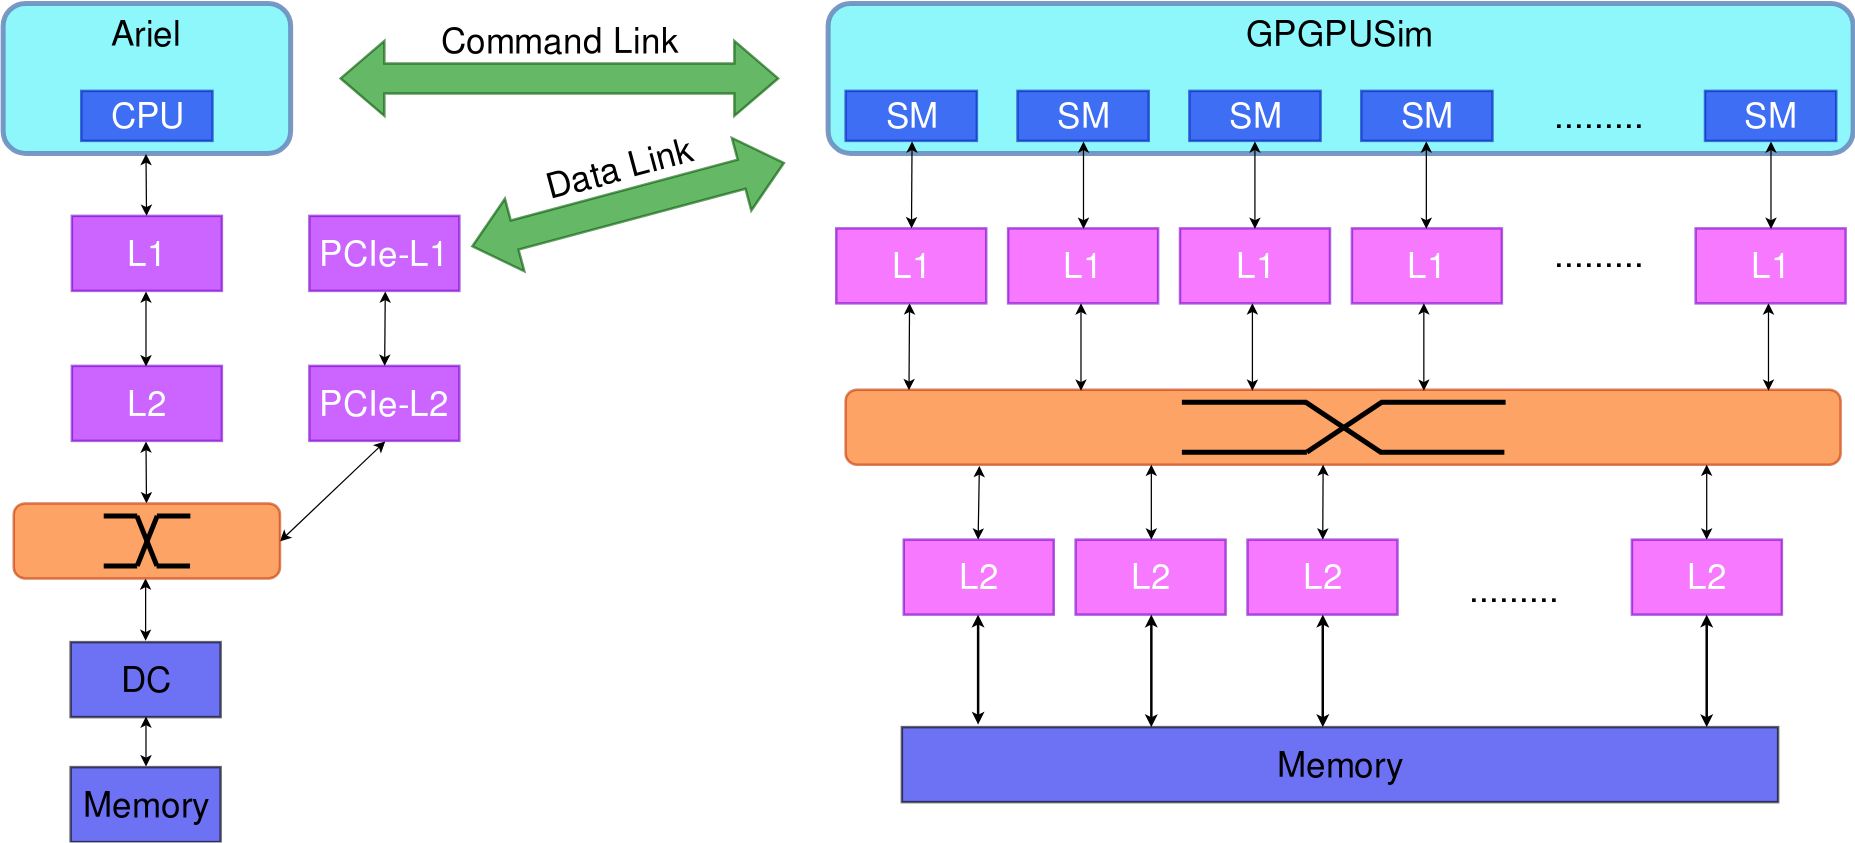
\includegraphics[width=.95\textwidth,keepaspectratio]{figures/sst_v100_model.png}
      \captionsetup{format=hang, justification=centering, width=.75\textwidth}
      \caption{SST Model of CPU With GPU Attached}
      \label{fig:sst_volta}
   \end{figure}

\section{Functional Testing}
The functional correctness of the model was validated using the unit tests from
the Kokkos Kernels suite~\cite{kokkos_kernels}. The unit tests were compiled
using the parameters in Table~\ref{tab:kokkos_build}. The target node
architecture was assumed to be an Intel Broadwell attached to an NVIDIA Pascal
GPUs. This target architecture was chosen based on hardware availability,
specifically Sandia's Doom cluster, which is based on the CTS-1
procurement. The SST model is derived from Figure~\ref{fig:sst_volta} using the
model parameters in Table`\ref{tab:p100_params} to represent an NVIDIA P100
SXM2~\cite{p100}.

    \begin{table}[!htbp]
        \centering
        \setlength{\abovecaptionskip}{6pt plus 1pt minus 1pt}
        \captionsetup{width=.75\textwidth}
        \caption{Kokkos Build Parameters}
        \begin{tabular}{|l|}
            \hline
            KOKKOSKERNELS\_SCALARS=double          \\ \hline
            KOKKOSKERNELS\_LAYOUTS=left            \\ \hline
            KOKKOSKERNELS\_ORDINALS=int            \\ \hline
            KOKKOSKERNELS\_OFFSETS=int             \\ \hline
            KOKKOSKERNELS\_DEVICES=Cuda     	   \\ \hline
            KOKKOS\_ARCH=Pascal60              	   \\ \hline
         \end{tabular}
        \label{tab:kokkos_build}
    \end{table}

    \begin{table}[!htbp]
      \centering
      \setlength{\abovecaptionskip}{6pt plus 1pt minus 1pt}
      \captionsetup{width=.75\textwidth}
      \caption{Broadwell/P100 Model Parameters}
      \subtable[CPU]{%
         \begin{tabular}{|l|c|}
            \hline
            Clock                   & 1200MHz  \\ \hline
            DDR Clock               & 2400     \\ \hline
            DDR Capactiy            & 16384MiB \\ \hline
            Mesh Frequency          & 800MHz   \\ \hline
            Mesh Input Ports        & 1        \\ \hline
            Mesh Output Ports       & 1        \\ \hline
            Data Link Latency       & 23840ps  \\ \hline
            Command Link Latency    & 23840ps  \\ \hline
         \end{tabular}
      }
      \hspace{1cm}
      \subtable[GPU]{%
         \begin{tabular}{|l|c|}
            \hline
            Clock                 & 1328MHz          \\ \hline
            SMs                   & 56               \\ \hline
            L2 Slices             & 8                \\ \hline
            L2 Capactiy           & 512KiB per slice \\ \hline
            HBM Capacity          & 16384MiB         \\ \hline
            HBM Stacks            & 4                \\ \hline
            Crossbar Frequency    & 1000MHz          \\ \hline
            Crossbar Input Ports  & 2                \\ \hline
            Crossbar Output Ports & 1                \\ \hline
         \end{tabular}
      }
      \label{tab:p100_params}
   \end{table}

Table~\ref{tab:kokkos_tests} shows the Kokkos Kernels unit tests that were run.
With the current implementation of SST-GPU, 38 out of 94 tests run to completion
and pass. The passing tests are highlighted in green. Of the remaining tests,
all but the yellow tests fail in both SST-GPGPU and GPGPU-Sim. The tests in pink
failed previously because the PTX parser cannot locate a post-dominator. Now since
the the target configuration for Kokkos compilation has been changed 
to aiming at only GPUs, these tests no longer exist. There
are plans to work with the Kokkos Kernels developers to find a solution. The
tests in purple fail because of a bug in the SST that causes double free. 
The SST developers should be able to locate the problem. The tests in red fail because
the final results are incorrect although they run to completion. Both teams are actively
engaged on a fix for this. The tests in blue did not exist previously but now fail 
because the current SST does not support cudaCreateTextureObject function. 
The two remaining tests, in yellow, run to completion
and pass in GPGPU-Sim but have run for more than 10 days without completion in SST. 
It is believed that they would complete successfully if given more run time.

   \begin{table}[!htbp]
      \centering
      \setlength{\belowcaptionskip}{6pt plus 1pt minus 1pt}
      \captionsetup{width=.75\textwidth}
      \caption{Kokkos Kernels Unit Test Results}
      \resizebox{\columnwidth}{!}{
         \begin{tabular}{|>{\columncolor[HTML]{34FF34}}l |l|}
            \hline
            1                          & abs\_double                                                         \\ \hline
            2                          & abs\_mv\_double                                                     \\ \hline
            3                          & asum\_double                                                        \\ \hline
            4                          & axpby\_double                                                       \\ \hline
            5                          & axpby\_mv\_double                                                   \\ \hline
            6                          & axpy\_double                                                        \\ \hline
            7                          & axpy\_mv\_double                                                    \\ \hline
            8                          & dot\_double                                                         \\ \hline
            9                          & dot\_mv\_double                                                     \\ \hline
            10                         & mult\_double                                                        \\ \hline
            11                         & mult\_mv\_double                                                    \\ \hline
            12                         & nrm1\_double                                                        \\ \hline
            13                         & nrm1\_mv\_double                                                    \\ \hline
            14                         & nrm2\_double                                                        \\ \hline
            15                         & nrm2\_mv\_double                                                    \\ \hline
            16                         & nrm2\_squared\_double                                               \\ \hline
            17                         & nrm2\_squared\_mv\_double                                           \\ \hline
            18                         & nrminf\_double                                                      \\ \hline
            19                         & nrminf\_mv\_double                                                  \\ \hline
            20 			       & reciprocal\_double                                                  \\ \hline
            21 			       & reciprocal\_mv\_double                                              \\ \hline
            22                         & scal\_double                                                        \\ \hline
            23                         & scal\_mv\_double                                                    \\ \hline
            24                         & sum\_double                                                         \\ \hline
            25                         & sum\_mv\_double                                                     \\ \hline
            26                         & update\_double                                                      \\ \hline
            27                         & update\_mv\_double                                                  \\ \hline
            \cellcolor[HTML]{F8FF00}28 & gemv\_double                                                        \\ \hline
            \cellcolor[HTML]{F8FF00}29 & gemm\_double                                                        \\ \hline
            \cellcolor[HTML]{FF00FF}30 & sparse\_spgemm\_double\_int\_int\_TestExecSpace                     \\ \hline
            \cellcolor[HTML]{FF00FF}31 & sparse\_spadd\_double\_int\_int\_TestExecSpace                      \\ \hline
            \cellcolor[HTML]{FF00FF}32 & sparse\_gauss\_seidel\_double\_int\_int\_TestExecSpace              \\ \hline
            \cellcolor[HTML]{FF00FF}33 & sparse\_block\_gauss\_seidel\_double\_int\_int\_TestExecSpace       \\ \hline
            \cellcolor[HTML]{FF00FF}34 & sparse\_crsmatrix\_double\_int\_int\_TestExecSpace                  \\ \hline
            \cellcolor[HTML]{FF00FF}35 & sparse\_blkcrsmatrix\_double\_int\_int\_TestExecSpace               \\ \hline
            \cellcolor[HTML]{FF00FF}36 & sparse\_replaceSumIntoLonger\_double\_int\_int\_TestExecSpace       \\ \hline
            \cellcolor[HTML]{FF00FF}37 & sparse\_replaceSumInto\_double\_int\_int\_TestExecSpace             \\ \hline
            \cellcolor[HTML]{FF00FF}38 & graph\_graph\_color\_double\_int\_int\_TestExecSpace                \\ \hline
            \cellcolor[HTML]{FF00FF}39 & graph\_graph\_color\_deterministic\_double\_int\_int\_TestExecSpace \\ \hline
            \cellcolor[HTML]{FF00FF}40 & graph\_graph\_color\_d2\_double\_int\_int\_TestExecSpace            \\ \hline
            \cellcolor[HTML]{FF00FF}41 & common\_ArithTraits                                                 \\ \hline
            42                         & common\_set\_bit\_count                                             \\ \hline
            43                         & common\_ffs                                                         \\ \hline
            \cellcolor[HTML]{FE0000}44 & batched\_scalar\_serial\_set\_double\_double                        \\ \hline
            \cellcolor[HTML]{FE0000}45 & batched\_scalar\_serial\_scale\_double\_double                      \\ \hline
            \cellcolor[HTML]{FE0000}46 & batched\_scalar\_serial\_gemm\_nt\_nt\_double\_double               \\ \hline
            \cellcolor[HTML]{D1B3FF}47 & batched\_scalar\_serial\_gemm\_t\_nt\_double\_double                \\ \hline
            \end{tabular}

            \hspace{1cm}

            \begin{tabular}{|>{\columncolor[HTML]{34FF34}}l |l|}
            \hline
            \cellcolor[HTML]{FE0000}48 & batched\_scalar\_serial\_gemm\_nt\_t\_double\_double                \\ \hline
            \cellcolor[HTML]{FE0000}49 & batched\_scalar\_serial\_gemm\_t\_t\_double\_double                 \\ \hline
            50                         & batched\_scalar\_serial\_trsm\_l\_l\_nt\_u\_double\_double          \\ \hline
            \cellcolor[HTML]{FE0000}51 & batched\_scalar\_serial\_trsm\_l\_l\_nt\_n\_double\_double          \\ \hline
            52                         & batched\_scalar\_serial\_trsm\_l\_u\_nt\_u\_double\_double          \\ \hline
            \cellcolor[HTML]{FE0000}53 & batched\_scalar\_serial\_trsm\_l\_u\_nt\_n\_double\_double          \\ \hline
            54                         & batched\_scalar\_serial\_trsm\_r\_u\_nt\_u\_double\_double          \\ \hline
            \cellcolor[HTML]{FE0000}55 & batched\_scalar\_serial\_trsm\_r\_u\_nt\_n\_double\_double          \\ \hline
            \cellcolor[HTML]{FF00FF}56 & batched\_scalar\_serial\_trsm\_l\_l\_t\_u\_double\_double           \\ \hline
            \cellcolor[HTML]{FF00FF}57 & batched\_scalar\_serial\_trsm\_l\_l\_t\_n\_double\_double           \\ \hline
            \cellcolor[HTML]{FF00FF}58 & batched\_scalar\_serial\_trsm\_l\_u\_t\_u\_double\_double           \\ \hline
            \cellcolor[HTML]{FF00FF}59 & batched\_scalar\_serial\_trsm\_l\_u\_t\_n\_double\_double           \\ \hline
            60                         & batched\_scalar\_serial\_gemv\_nt\_double\_double                   \\ \hline
            61                         & batched\_scalar\_serial\_gemv\_t\_double\_double                    \\ \hline
            \cellcolor[HTML]{FE0000}62 & batched\_scalar\_serial\_trsv\_l\_nt\_u\_double\_double             \\ \hline
            \cellcolor[HTML]{FE0000}63 & batched\_scalar\_serial\_trsv\_l\_nt\_n\_double\_double             \\ \hline
            \cellcolor[HTML]{FE0000}64 & batched\_scalar\_serial\_trsv\_u\_nt\_u\_double\_double             \\ \hline
            \cellcolor[HTML]{FE0000}65 & batched\_scalar\_serial\_trsv\_u\_nt\_n\_double\_double             \\ \hline
            \cellcolor[HTML]{FE0000}66 & batched\_scalar\_team\_set\_double\_double                          \\ \hline
            \cellcolor[HTML]{FE0000}67 & batched\_scalar\_team\_scale\_double\_double                        \\ \hline
            \cellcolor[HTML]{D1B3FF}68 & batched\_scalar\_team\_gemm\_nt\_nt\_double\_double                 \\ \hline
            \cellcolor[HTML]{D1B3FF}69 & batched\_scalar\_team\_gemm\_t\_nt\_double\_double                  \\ \hline
            \cellcolor[HTML]{FE0000}70 & batched\_scalar\_team\_gemm\_nt\_t\_double\_double                  \\ \hline
            \cellcolor[HTML]{D1B3FF}71 & batched\_scalar\_team\_gemm\_t\_t\_double\_double                   \\ \hline
            72                         & batched\_scalar\_team\_trsm\_l\_l\_nt\_u\_double\_double            \\ \hline
            \cellcolor[HTML]{FE0000}73 & batched\_scalar\_team\_trsm\_l\_l\_nt\_n\_double\_double            \\ \hline
            74                         & batched\_scalar\_team\_trsm\_l\_u\_nt\_u\_double\_double            \\ \hline
            \cellcolor[HTML]{FE0000}75 & batched\_scalar\_team\_trsm\_l\_u\_nt\_n\_double\_double            \\ \hline
            76                         & batched\_scalar\_team\_trsm\_r\_u\_nt\_u\_double\_double            \\ \hline
            \cellcolor[HTML]{FE0000}77 & batched\_scalar\_team\_trsm\_r\_u\_nt\_n\_double\_double            \\ \hline
            \cellcolor[HTML]{FF00FF}78 & batched\_scalar\_team\_trsm\_l\_l\_t\_u\_double\_double             \\ \hline
            \cellcolor[HTML]{FF00FF}79 & batched\_scalar\_team\_trsm\_l\_l\_t\_n\_double\_double             \\ \hline
            \cellcolor[HTML]{FF00FF}80 & batched\_scalar\_team\_trsm\_l\_u\_t\_u\_double\_double             \\ \hline
            \cellcolor[HTML]{FF00FF}81 & batched\_scalar\_team\_trsm\_l\_u\_t\_n\_double\_double             \\ \hline
            82                         & batched\_scalar\_team\_gemv\_nt\_double\_double                     \\ \hline
            83                         & batched\_scalar\_team\_gemv\_t\_double\_double                      \\ \hline
            \cellcolor[HTML]{FE0000}84 & batched\_scalar\_serial\_lu\_double                                 \\ \hline
            \cellcolor[HTML]{FF00FF}85 & batched\_scalar\_serial\_inverselu\_double                          \\ \hline
            \cellcolor[HTML]{FF00FF}86 & batched\_scalar\_serial\_solvelu\_double                            \\ \hline
            \cellcolor[HTML]{D1B3FF}87 & batched\_scalar\_team\_lu\_double                                   \\ \hline
            \cellcolor[HTML]{FF00FF}88 & batched\_scalar\_team\_inverselu\_double                            \\ \hline
            \cellcolor[HTML]{FF00FF}89 & batched\_scalar\_team\_solvelu\_double                              \\ \hline
            \cellcolor[HTML]{0000FF}90 & sparse\_spmv\_double\_int\_int\_TestExecSpace                            \\ \hline
	    \cellcolor[HTML]{0000FF}91 & sparse\_spmv\_mv\_double\_int\_int\_LayoutLeft\_TestExecSpace              \\ \hline
	    \cellcolor[HTML]{0000FF}92 & sparse\_spmv\_mv\_double\_int\_int\_LayoutRight\_TestExecSpace             \\ \hline
	    \cellcolor[HTML]{0000FF}93 & sparse\_trsv\_mv\_double\_int\_int\_LayoutLeft\_TestExecSpace              \\ \hline
	    \cellcolor[HTML]{0000FF}94 & sparse\_trsv\_mv\_double\_int\_int\_LayoutRight\_TestExecSpace             \\ \hline 
	\end{tabular}}
      \label{tab:kokkos_tests}
   \end{table}




\section{Correlation with Volta}
A validation sweep was run using six benchmarks. These
applications were run using UVM Smart model that approximates a Nvidia V100. The simulation parameters are shown in Table
\ref{tab:v100_params}. The overall kernel runtime was compared with the results
of running the six applications through nvprof on Nvidia Tesla V100. Figure \ref{fig:correlation}
shows the total number cycles that each application took on the simulation model
and on the native V100. Note that this is only cycles where a kernel was running
and does not include host execution time. The performance gap mainly comes from prefetching algorithms. The blue cross points represent the result of no prefetcher applied, the yellow represents random prefetched, the black represents the sequential locality prefetcher, and the cyan represents the tree-based neighbor prefetcher. It is very clear that the tree-based neighbor prefetcher has the best correlation, which seems very close to the tree-based hardware prefetcher implemented by NVIDIA CUDA driver.

   \begin{figure}[!htb]
      \centering
      \setlength{\abovecaptionskip}{6pt plus 1pt minus 1pt}
      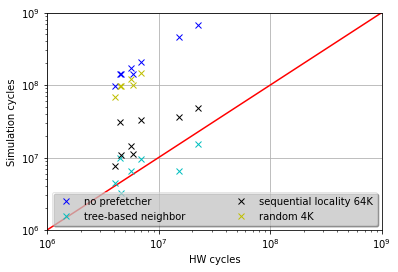
\includegraphics[width=.90\textwidth,keepaspectratio]{figures1/corre.elf}
      \captionsetup{width=.75\textwidth}
      \caption{Correlations between simulator and hardware.}
      \label{fig:correlation}
   \end{figure}


    \begin{table}[!htbp]
      \centering
      \setlength{\belowcaptionskip}{6pt plus 1pt minus 1pt}
      \captionsetup{width=.75\textwidth}
      \caption{CPU/V100 Model Parameters}
      \hspace{1cm}
         \begin{tabular}{|l|c|}
            \hline
            Clock                 & 1312MHz          \\ \hline
            SMs                   & 84               \\ \hline
            L2 Slices             & 32               \\ \hline
            L2 Capactiy           & 192KiB per slice \\ \hline
            HBM Capacity          & 16384MiB         \\ \hline
            HBM Stacks            & 4                \\ \hline
            Crossbar Frequency    & 1200MHz          \\ \hline
            Crossbar Input Ports  & 2                \\ \hline
            Crossbar Output Ports & 1                \\ \hline
         \end{tabular}
      \label{tab:v100_params}
   \end{table}

\section{Lulesh Performance Study}
A parameter sweep was performed using LULESH, described in Section
\ref{sec:lulesh}. The device clock was varied from 500MHz to 1312MHz to 1800MHz.
The memory clock was varied from 877MHz to 1200MHz to 1600MHz. Figure
\ref{fig:lulesh_sweep} shows the results, where lower runtime time is better.


As expected, changing the frequency of the backing store has little effect on
LULESH for this problem size because it is not memory bandwidth bound. The most
improvement is seen at the low device clock frequency, but at this frequency
the speedup is still small at 1.04x.
However, increasing the frequency of the SMs does improve the
performance noticeably. Going from 500MHz to 1312MHz shows a 2.5x speedup; going
from 1312MHz to 1800MHz shows a further 1.3x speedup.

Although this was a small study, one can imagine being able to run a more
complete parameter sweep over any of the Balar parameters.

   \begin{figure}[!htb]
      \centering
      \setlength{\abovecaptionskip}{6pt plus 1pt minus 1pt}
      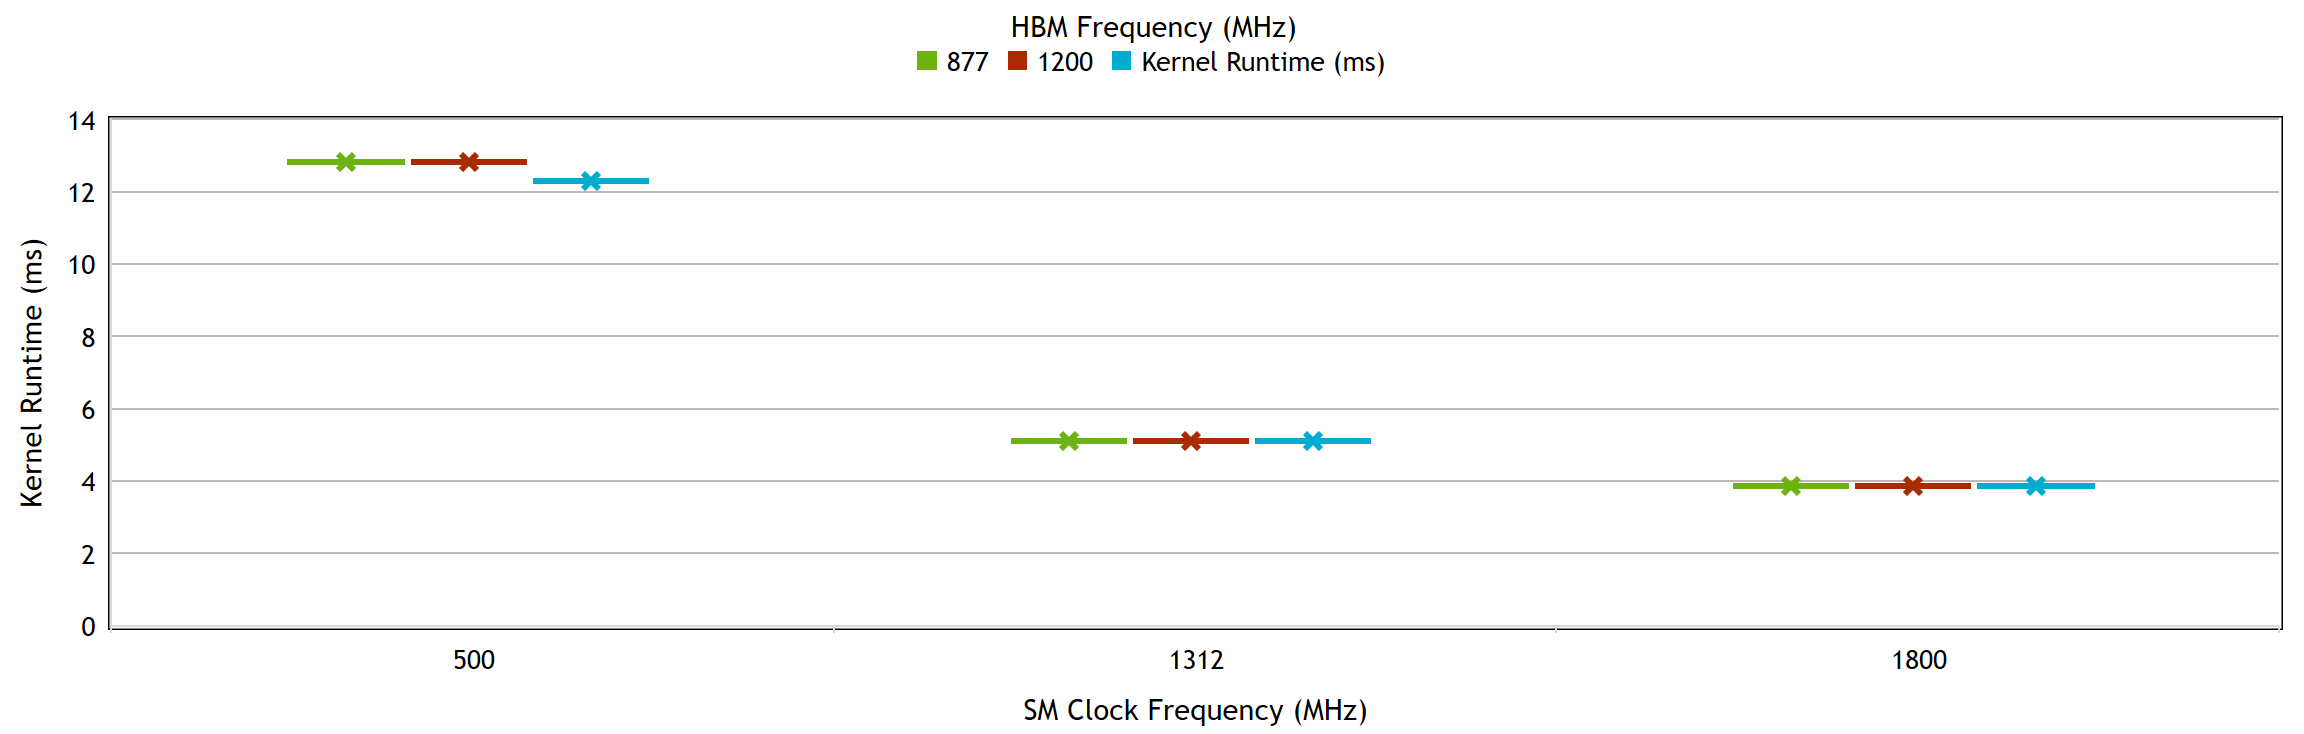
\includegraphics[width=.98\textwidth,keepaspectratio]{figures/lulesh_sweep.png}
      \captionsetup{format=hang, justification=centering, width=.75\textwidth}
      \caption[GPU Parameter Sweep Using LULESH]{GPU Parameter Sweep Using LULESH\\(Baseline was 1312MHz/877MHz)}
      \label{fig:lulesh_sweep}
   \end{figure}


% Design space exploration is not the only use case for this integration. One of
% the more novel features of SST is the ability to obtain periodic statistic dumps
% for all of the currently loaded components. This presents enormous opportunities
% for system designers and application developers. Modern performance profiling
% tools can only provide users with, relatively, coarse-grain details from
% performance counters. SST can provide statistics for any component in the model
% at a time granularity defined by the user. The plots in the figures below are
% all at a 2us granularity. Imagine being able to query that information on any
% time scale for any of the ~20k component statistics in this model! Figure
% \ref{fig:time_sweep} shows an example of this with the host activity plotted in
% \ref{fig:host_cycles} and the GPU crossbar activity plotted in
% \ref{fig:crossbar_activity} (used here as a stand-in for GPU activity).
%
% Kernel launches are asynchronous with the host unless explicitly declared otherwise.
% Even memory copies from the host to the device are asynchronous in this model -- the
% scheduling unit queues all work from a given stream and can guarantee correctness.
%
%    \begin{figure}[!htb]
%       \centering
%       \setlength{\abovecaptionskip}{6pt plus 1pt minus 1pt}
%       \subfigure[Host Cycles]{
%          \label{fig:host_cycles}
%          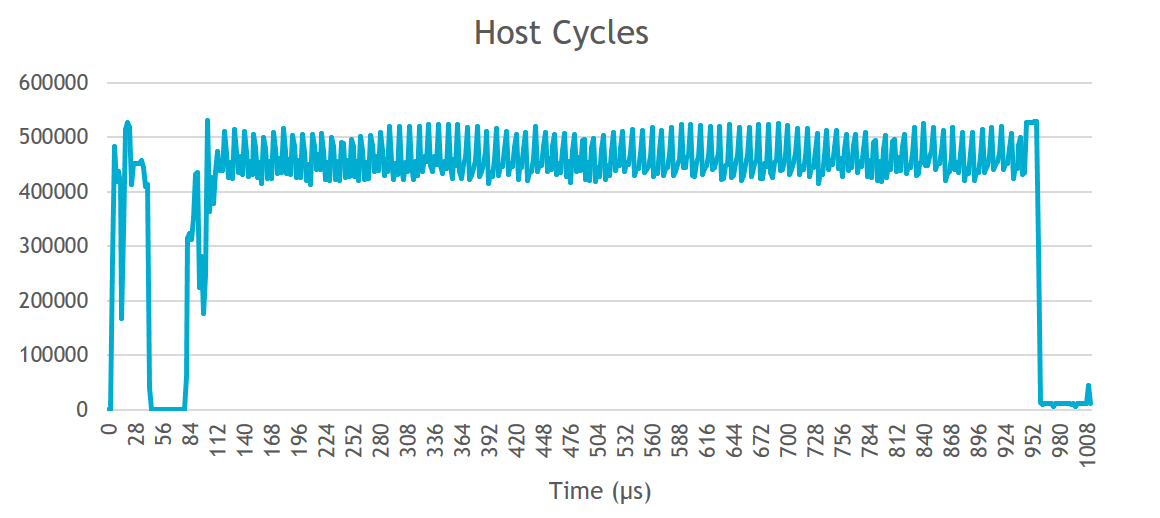
\includegraphics[width=.48\textwidth,height=4cm]{figures/host_cycles.png}
%       }
%       \subfigure[Device Crossbar Activity]{
%          \label{fig:crossbar_activity}
%          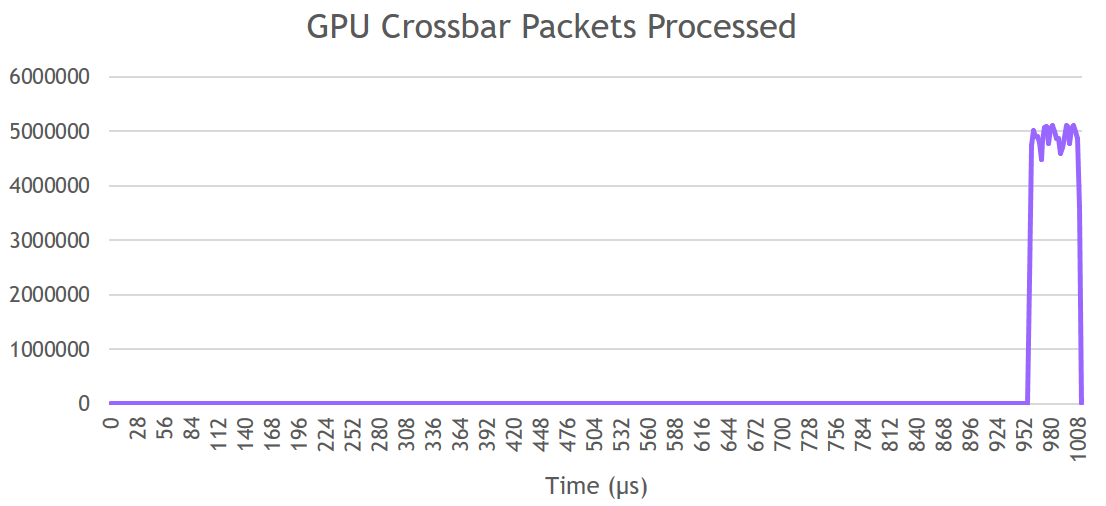
\includegraphics[width=.48\textwidth,height=4cm]{figures/crossbar_packets.png}
%       }
%       \caption{Full caption.}
%       \label{fig:time_sweep}
%    \end{figure}

